\documentclass[10pt,a4paper]{report}
\newcommand{\confdir}{../conf/} % Set the folder which contains preamble.tex, titlepage.tex and the general img/ folder
\newcommand{\imgdir}{img/} % Set the folder which contains the specific images for the report
\newcommand{\texdir}{tex/} % Set the folder which contains the content (.tex files)
\input{\confdir preamble}


%%%%%%%%%%%
%% SETUP %%
%%%%%%%%%%%

%% Set the course number and course name
% Usage: \setcourse{<course no>}{<course name>}
	\setcourse{02450}{Introduction to Machine Learning and Data Modeling}

%% Set the title of the report
% Usage: \settitle{<title>}
	\settitle{Assignment 1}

%% Set the subtitle of the report
% Usage: \setsubtitle{<subtitle>}
	\setsubtitle{Feature Extraction and Visualization}

%% Set the date the report is handed in
% Usage: \setdate{<hand-in date>}
	\setdate{March 5th 2013}

%% Add the authors of the report
% Usage: \addauthor{<study number>}{<first name(s)>}{<last name>}
	\addauthor{s093294}{Poul Kjeldager}{Sørensen}
	\addauthor{s093280}{Martin Kasban}{Tange}

%%%% END OF SETUP

%ADDED BY POUL
\renewcommand{\topfraction}{0.85}
\renewcommand{\textfraction}{0.1}
\renewcommand{\floatpagefraction}{0.75}
\usepackage[draft,english,margin]{fixme}




\begin{document}

%% Insert titlepage
\inserttitlepage

%% Insert table-of-contents
\inserttoc

%% Input files for the report
\input{\texdir introduction}

\chapter{Data and Feature Extraction}
%What is the problem of interest.
%Where did we obtain the data.(already answered)
%What have been done to the data before(A lot, but havent written much about it. People are using it still for benchmarks and people are down to less than 40 errors of the 10000 test examples))
%Explain what the primary machien learning modeling aim is as well as how you envision the data can be analysed in therms of; a classification, a regression a clustering, and association mining and an anomaly detection problem. (You need to outline how all the methods may be applied to your data)

\section{Introduction}
In this chapter the data are presented and how the features have been extracted are outlined.
\input{\texdir intro_feature_extraction}
\input{\texdir intro_machine_learning} 

\chapter{Data Analysis}
%A detailed explanation of the attributes of the data. discrete/continos, nominal/ordinal/interval/radio). Data issues like missing values, corrupted data. The basic summary statistics of the attributes.

\section{Introduction}
In this chapter a detailed explanation of the attributes will be given. It will be shown how the attributes are somewhat correlated and the real dimensionality of the data will be found using Principal Component Analysis (PCA). 

\section{Basic Statistic Properties}
By means of the ACCENT\footnote{Apprehension, clarity, consistency, efficiency, necessity and truthfulness} principles some interesting figures have been made in Matlab to illustrate some properties of the data. Some summary statistics have also been omitted as them not contributing any further information for this dataset. An example of this is computing the mean and standard deviation(std). Instead the std have been computed from standardized data, for 2000 randomly drawn samples, and plotted in Figure~\ref{fig:1b}. 
 
\begin{figure}[hbtp]
\begin{minipage}[t]{.49\linewidth}
\centering
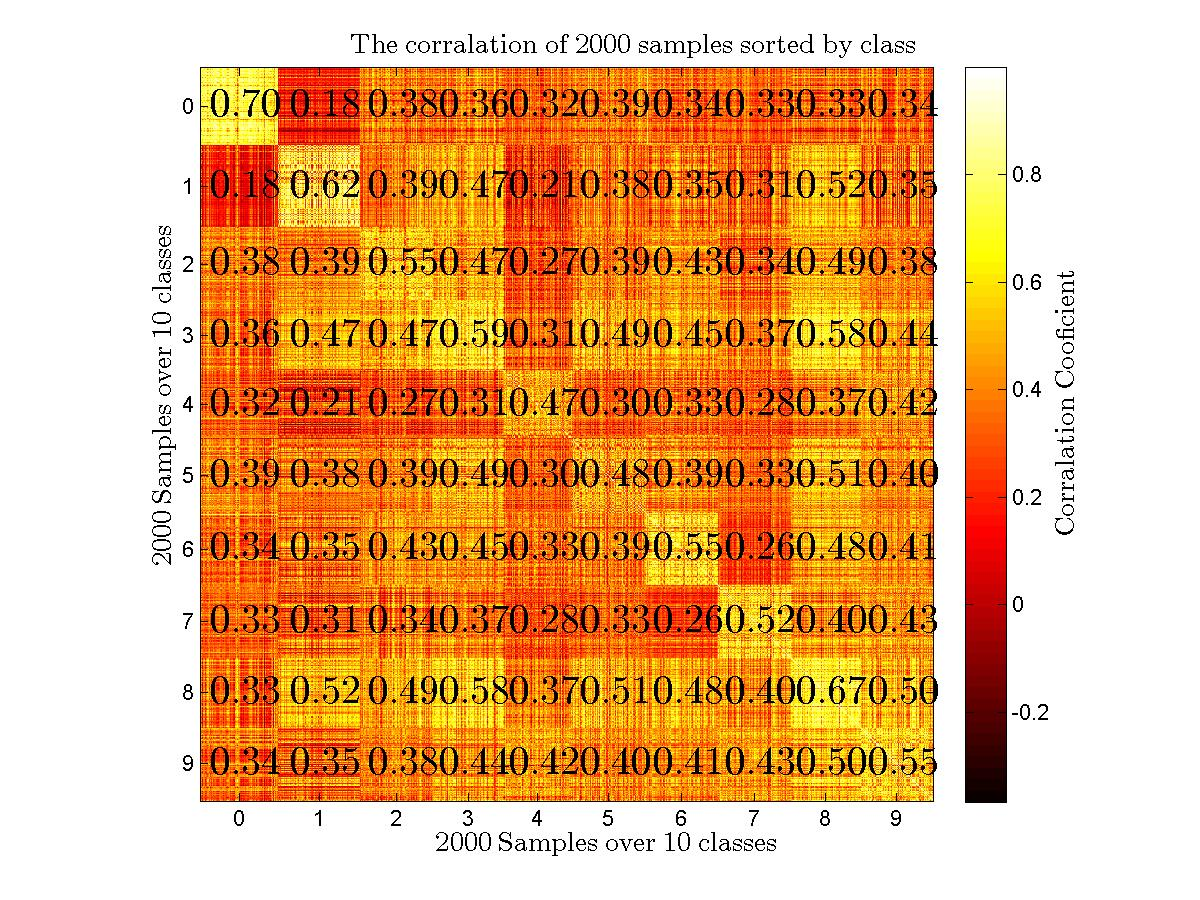
\includegraphics[width=\linewidth]{corr_explained}
\subcaption{The correlation of 2000 randomly drawn samples sorted by class. The mean of each class-by-class square have its mean value printed ontop. \label{fig:1a}}
\end{minipage}%
\hfill%
\begin{minipage}[t]{.49\linewidth}
\centering
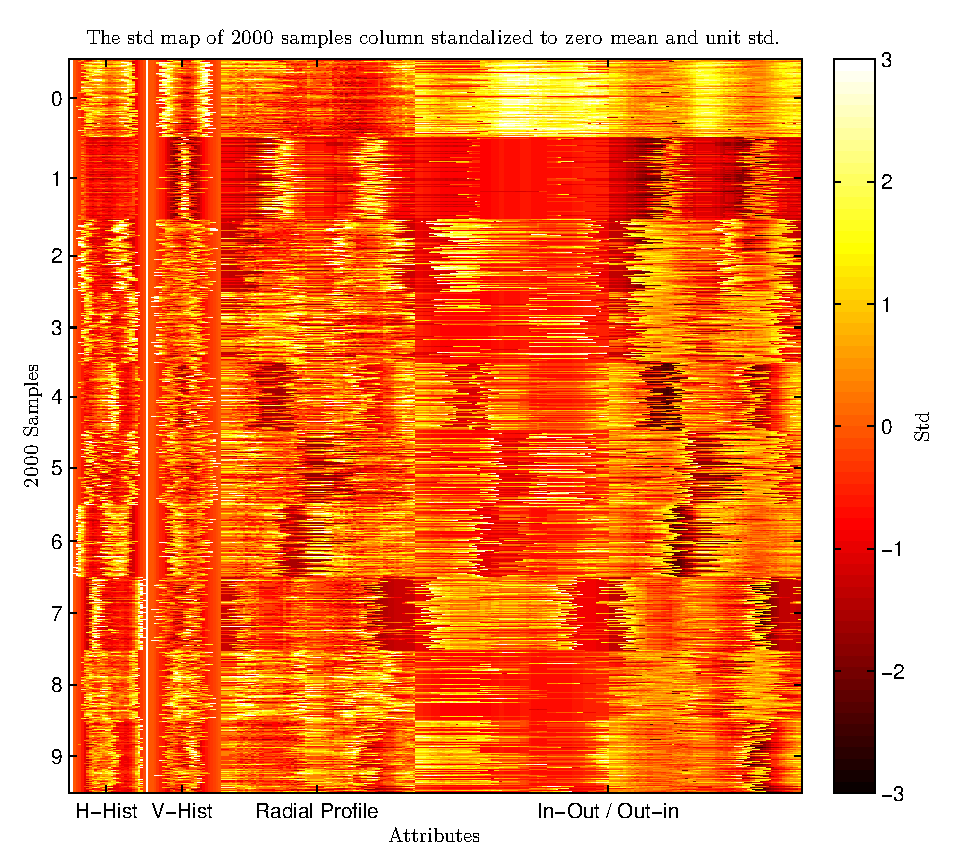
\includegraphics[width=\linewidth]{std_explained}
\subcaption{The std of all attributes from the same 2000 samples in Figure~\ref{fig:1a}. \label{fig:1b}}
\end{minipage}
\caption{Conclusion: Classes are clearly correlated and it should be possible to apply classification routines to separate the classes. }
\end{figure}

From Figure~\ref{fig:1b} some properties can be seen. One example would be the class of zeros in-out profile are significant higher than the average and classes of ones have its horizontal histogram below average near the middle and higher in the middle. Keeping this information in mind and returning to Figure~\ref{fig:image_examples} this becomes truth when looking at the features. The ten zeros shown earlier have a medium respond for the in-out profile while the five other classes have almost zeros. It also makes sense that ones have high response at the middle because of ones being vertical lines and nothing around them.

\subsection{Correlation}
In Figure~\ref{fig:1a} the correlation of samples have been computed ans sorted by classes. Further more the mean value for each class by class square box have been computed and plotted on top for truthfulness when colours fails. It can been seen that classes has some correlation with the other classes, but important is that each class is mostly correlated with its own class.

\begin{figure}[hbtp]
\centering
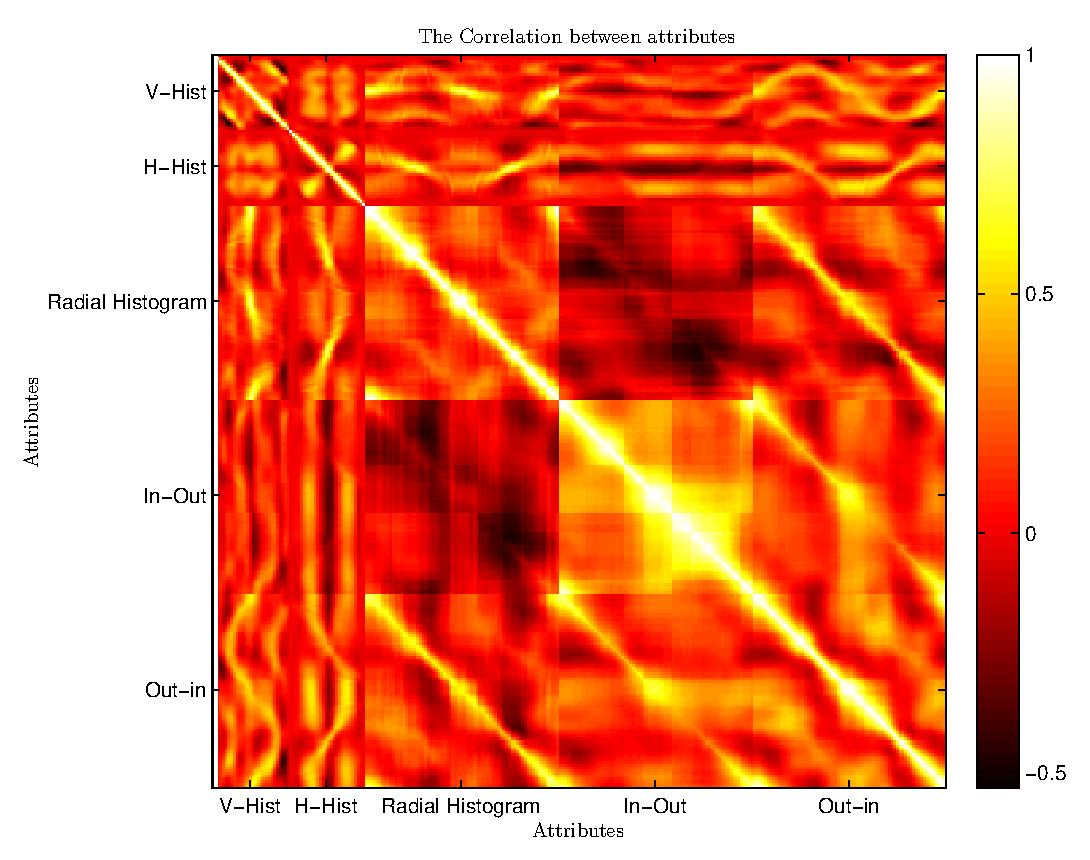
\includegraphics[width=0.49\linewidth]{att_corr_explained}
\caption{The correlation of attributes. Conclusion: Highly correlated and dimension can be reduced.\label{fig:att_corr_explained}}
\end{figure}

It can also be very interesting to look at correlation between attributes, as shown in Figure~\ref{fig:att_corr_explained}. Its seen that the attributes are highly correlated in parts of the plot and it also make sense when looking back on the feature generation. The histograms correlate and some kind of symmetry is shown in the figure. This could very well be explained by the fact that a lot of the digits actually also have symmetric parts. Instead of speculating in such relationships, a PCA will be used to find the real dimension of the data.  


\section{Principal Component Analysis}
\fixme{The amount of variation explained as a function of the number of PCA com- ponents included}
\fixme{the principal directions of the considered PCA components}
\fixme{the data projected onto the considered principal components}
\input{\texdir pca}

\chapter{Discussion}
%What have we learned about the data.

\section{Conclusion}
%Summarize that we have included all the relevant information from the questions raised in the assignment text and tell how good a job we have done.

\bibliography{\confdir final}
\bibliographystyle{plain}


\end{document}
